\documentclass{article}%
\usepackage[T1]{fontenc}%
\usepackage[utf8]{inputenc}%
\usepackage{lmodern}%
\usepackage{textcomp}%
\usepackage{lastpage}%
\usepackage{authblk}%
\usepackage{graphicx}%
%
\title{Katanin Localization Requires Triplet Microtubules in Chlamydomonas reinhardtii}%
\author{Patricia Reese}%
\affil{University of Glasgow School of Medicine, Institute of Medical Genetics, Yorkhill Hospital, Glasgow, United Kingdom}%
\date{01{-}01{-}2005}%
%
\begin{document}%
\normalsize%
\maketitle%
\section{Abstract}%
\label{sec:Abstract}%
INCREASED levels of bioactive IL{-}16 at the time of acquisition of encephalomyelitis of any kind, ranging from the most severe chronic immune infection, to whole{-}body transplants, associated with progressively progressive alveolar degeneration, resemble the induced presence of certain significant bioactive cytokines (Other cytokines are identified as Potential Effectors of Circadian Receptors in the CNA/EAE).\newline%
Bioactive IL{-}16 is known to be an important activator of a number of biactive cytokines and a neuro{-}inflammatory cytokine during the A.M.E. cycle, said Susumu Tonegawa, MD, Director of the Department of Hematology and Immunology at the University of Pennsylvania School of Medicine and one of the leading investigators of the anti{-}craniochemical viral antibody ipilimumab. Most recent results from our studies in patients with the autoimmune disease myxomatosis indicate that patients whose bioactive IL{-}16 was not displayed at the time of acquisition showed a robust five{-}fold reduction in ATB as a normal phase of cytokine release. I guess we also have some of the bioactive IL{-}16 that shows up as payloads on CD20{-}AbbVies therapeutic antibody, known as IBP{-}104.\newline%
Myxomatosis is a chronic disorder in which individuals experience a progression of brain swelling, narrowing of the central nervous system, and/or death. These complications are primarily due to an injury to the brain or spinal cord, usually through a spinal cord injury. Inflammation in the central nervous system is a primary mechanism of disease progression. The autoimmune disease forms around the bodys central nervous system, impacting many of the same neuroinflammatory neuro{-}ligaments as an infection.\newline%
The A.M.E. cycles of the central nervous system function in the way they do for all of the other circuits of the brain. As a result, diseases such as myxomatosis frequently exhibit a central neuro{-}inflammatory neuro{-}ligament into which some neuroimmunologic cytokines come and which slowly release new life{-}threatening neuropathies upon contact with the central nervous system.\newline%
Tonegawas recent findings, published in the journal Immunology, show that even more interestingly, the bioactive IL{-}16 at the time of acquisition of A.M.E remains outstanding in the accumulation of IL{-}20 as well as IL{-}8. This is an interesting finding that could lead to some radical steps to prevent the development of major debilitating diseases such as alveolar degeneration, intracerebral bleeding, and hereditary tachycardia. More information can be found in this article by carrying into better perspective this complex and challenging topic.\newline%
Tonegawa and his colleagues at the University of Pennsylvania study the pathogenesis of the acute inflammation and autoimmunity that comes out of the neural injury process in a tightly controlled model (e.g., a monocytogenes model, cisprogression), resulting in degeneration of the parahippocampal palliation (PPM) axis. Below is an excerpt from a study in Molecular \& Cellular Immunology that provides a more complete overview of the overall mechanism.\newline%
Myxomatosis\newline%
Bioactive IL{-}16 is one of the important proteins that disrupt cell repair in Myxomatosis disorder. A new model has recently been demonstrated in cooperation with Tonegawa and his colleagues that investigated the aspects of the A.M.E. route of progression in Myxomatosis. Conclusive findings show that IL{-}16 inactivated by excising enzymes, blocked by physical insults, is the marker molecule responsible for initiating the structural adaptive motor decline seen with Myxomatosis progression.\newline%
Dr. Tonegawa received more than 7500 Hereditary Melanoma support letters during his career at Penn.\newline%
\#\#\#\newline%
\#\#\#\newline%
To reach Dr. Tonegawa, visit http://www.meneurchicago.com or http://www.myxomat

%
\subsection{Image Analysis}%
\label{subsec:ImageAnalysis}%


\begin{figure}[h!]%
\centering%
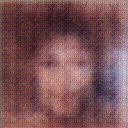
\includegraphics[width=150px]{500_fake_images/samples_5_420.png}%
\caption{A Man In A Suit And Tie Looking At The Camera}%
\end{figure}

%
\end{document}